% Fase 3B, exemplos 13–14. Fontes: mb-uso/secoes.
\begin{frame}[fragile]{Exemplo 13 — GD, IGD e EMD não perguntam a mesma coisa}
\textbf{DTLZ2 bidimensional, uma execução de NSGA-II.}
\begin{columns}[T,onlytextwidth]
\begin{column}{.45\textwidth}
\begin{lstlisting}[style=python,basicstyle=\ttfamily\fontsize{7.7}{9.6}\selectfont]
igd = mb.metrics.igd(exp)
gd  = mb.metrics.gd(exp)
emd = mb.metrics.emd(exp)
print(igd.last, gd.last, emd.last)
mb.view.history(igd, gd, emd)
\end{lstlisting}
\end{column}
\begin{column}{.53\textwidth}
\textbf{GD:} quão longe estão os pontos obtidos de sua referência mais próxima? \emph{Convergência.}
\par\smallskip
\textbf{IGD:} quão longe estão os pontos de referência das soluções obtidas? \emph{Cobertura e proximidade.}
\par\smallskip
\textbf{EMD:} qual o custo de redistribuir a massa de pontos entre os conjuntos? \emph{Distribuição.}
\end{column}
\end{columns}
\vspace{.13cm}\textbf{Por exemplo:} uma aproximação concentrada em uma pequena região ótima pode ter GD baixo, mas IGD e EMD elevados porque deixa outras regiões da frente pouco representadas.
\end{frame}

\begin{frame}{Exemplo 13 — Três trajetórias complementares de melhora}
\begin{columns}[T,onlytextwidth]
\begin{column}{.65\textwidth}
\centering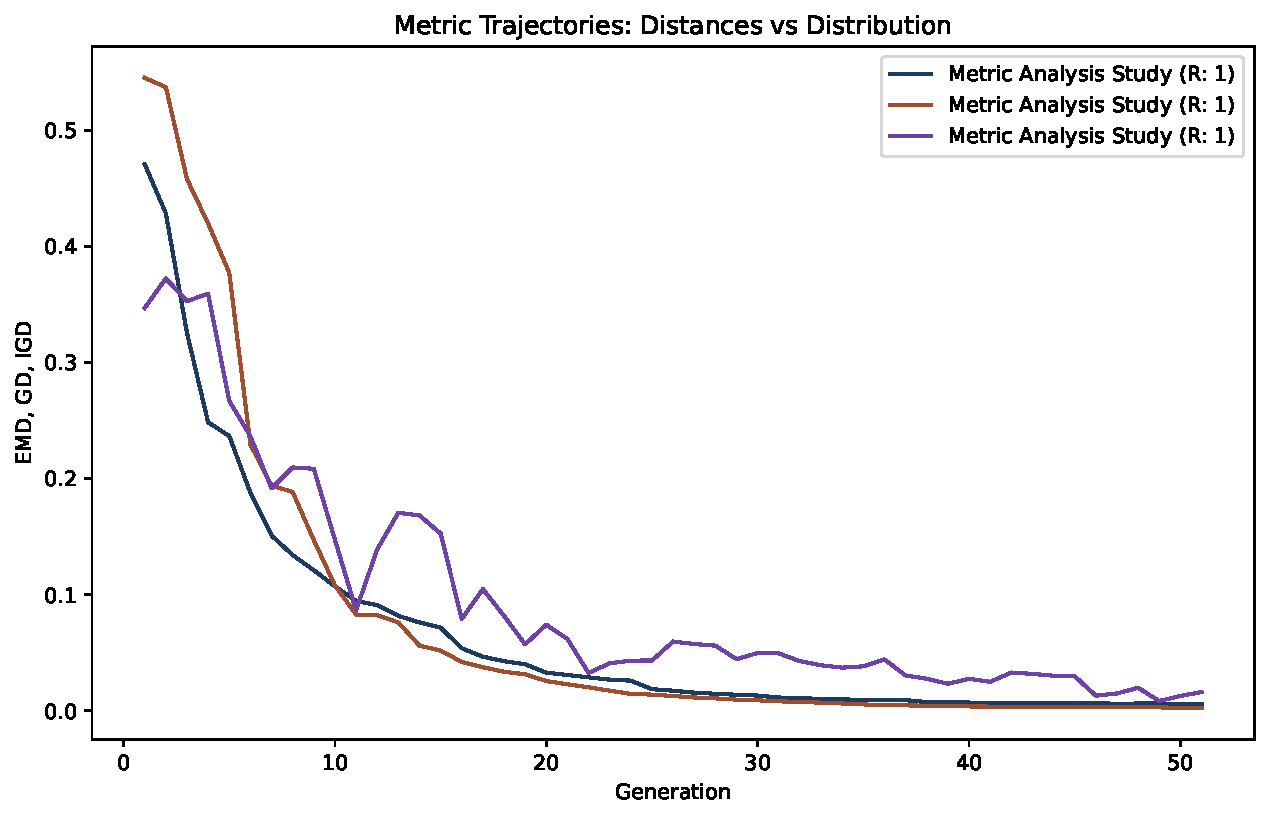
\includegraphics[width=\linewidth,height=.60\textheight,keepaspectratio]{figures/example_17_02_history.pdf}
\end{column}
\begin{column}{.33\textwidth}
\textbf{Primeira $\to$ última geração}
\par\smallskip
GD: \textbf{0,545305 $\to$ 0,002331}
\par\smallskip
IGD: \textbf{0,470870 $\to$ 0,005899}
\par\smallskip
EMD: \textbf{0,346937 $\to$ 0,015964}
\end{column}
\end{columns}
\vspace{.05cm}\textbf{Interpretação:} a GD aponta aproximação à referência; a IGD indica redução das regiões mal cobertas; a EMD mostra melhora da correspondência distributiva. Não são três maneiras equivalentes de medir o mesmo fenômeno.
\end{frame}

\begin{frame}[fragile]{Exemplo 14 — Comparar o HV métrico ao HV ordinal}
\textbf{DTLZ2 com 3 objetivos, três execuções de NSGA-II e três de NSGA-III.} A referência é compartilhada.
\begin{columns}[T,onlytextwidth]
\begin{column}{.48\textwidth}
\begin{lstlisting}[style=python,basicstyle=\ttfamily\fontsize{7.2}{9}\selectfont]
ref = [exp1, exp2]
hv1 = mb.metrics.hv(
    exp1, ref=ref, mode='exact')
hv2 = mb.metrics.hv(
    exp2, ref=ref, mode='exact')
oh1 = mb.metrics.ohv(
    exp1, ref=ref, mode='exact')
oh2 = mb.metrics.ohv(
    exp2, ref=ref, mode='exact')
\end{lstlisting}
\end{column}
\begin{column}{.50\textwidth}
\textbf{Diferença conceitual}
\par\smallskip
\textbf{HV:} preserva distâncias numéricas entre valores dos objetivos.
\par\smallskip
\textbf{OHV:} usa passos ordinais de mesmo peso entre níveis consecutivos da referência, independentemente do tamanho numérico dos intervalos.
\par\medskip
\textbf{Pergunta:} a superioridade permanece quando passamos da geometria métrica à ordem dos valores?
\end{column}
\end{columns}
\end{frame}

\begin{frame}{Exemplo 14 — Resultado nas duas escalas}
\begin{columns}[T,onlytextwidth]
\begin{column}{.49\textwidth}
\centering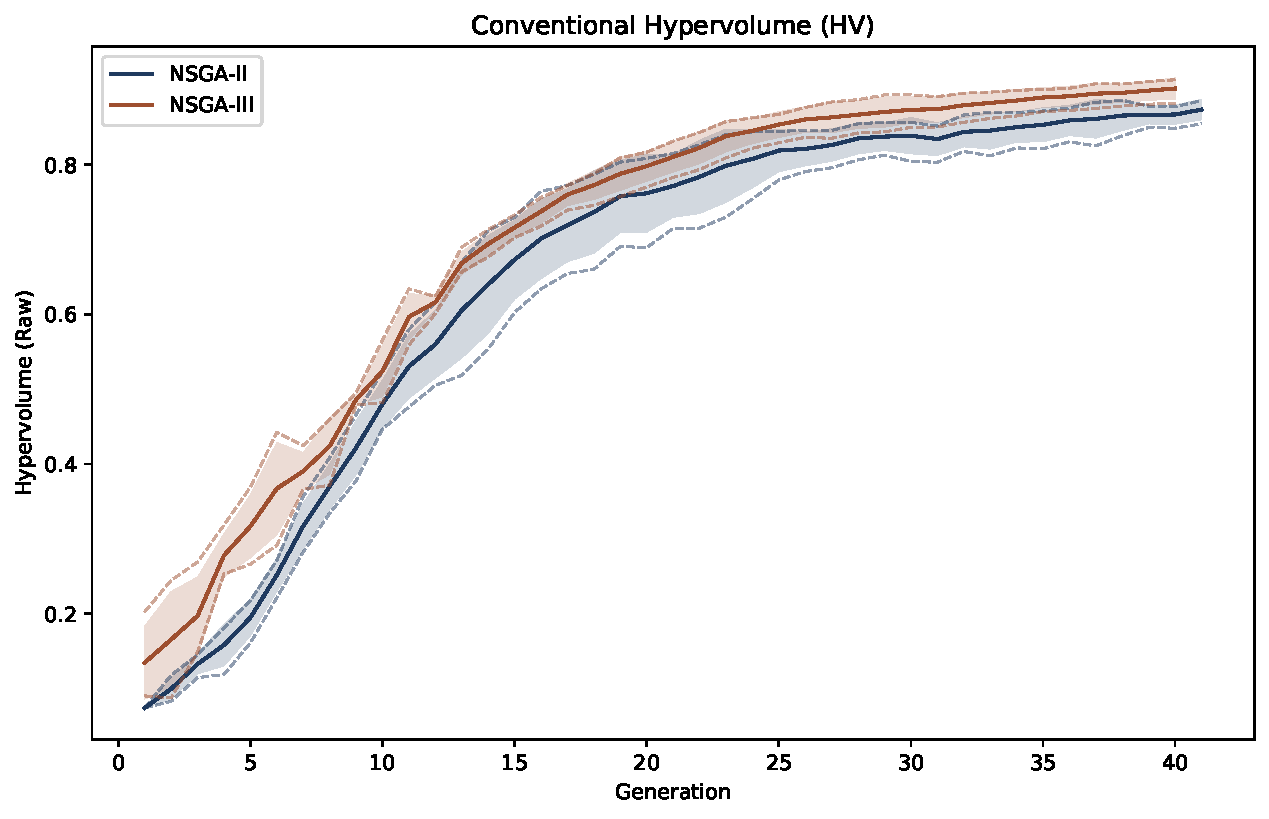
\includegraphics[width=\linewidth,height=.43\textheight,keepaspectratio]{figures/example_19_01_history.pdf}
\par{\scriptsize HV convencional (média final).}
\par\smallskip
NSGA-II: \textbf{0,873786} \quad NSGA-III: \textbf{0,901957}
\end{column}
\begin{column}{.49\textwidth}
\centering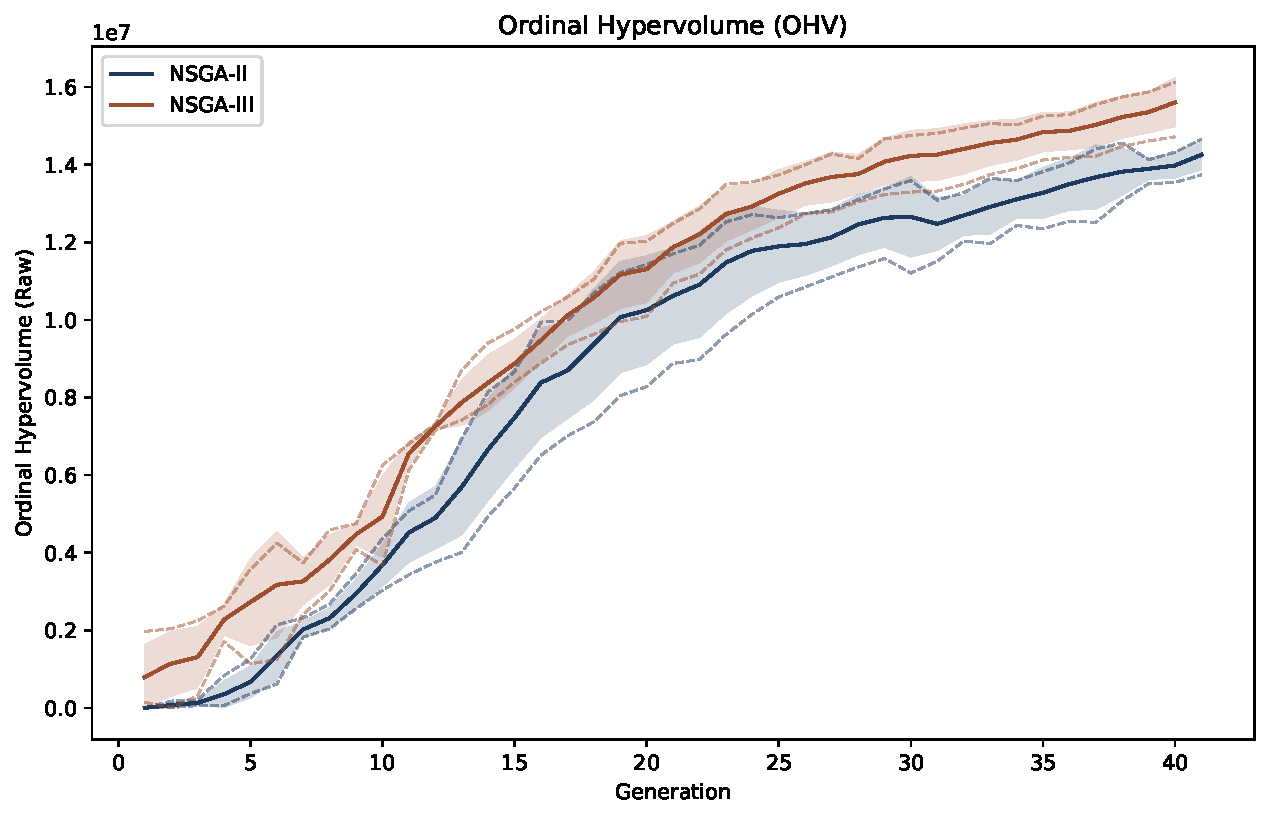
\includegraphics[width=\linewidth,height=.43\textheight,keepaspectratio]{figures/example_19_02_history.pdf}
\par{\scriptsize OHV (média final, unidades ordinais).}
\par\smallskip
NSGA-II: \textbf{14.254.117}
\par NSGA-III: \textbf{15.603.097}
\end{column}
\end{columns}
\vspace{.16cm}\textbf{Interpretação:} neste experimento, NSGA-III termina acima de NSGA-II em ambas as avaliações. A diferença não depende exclusivamente dos tamanhos numéricos dos intervalos entre objetivos; também permanece na régua ordinal.
\end{frame}